\chapter{Construction Notes}

\section{Components and Layout}

The following is a 'bill of materials' (BOM) needed to populate the D13 data separator. The component layout is shown in \textbf{Fig. \ref{fig:layout}}.

\begin{verbatim}
    C1   0.1 uF
    C2   0.1 uF
    C3   0.1 uF
    C34  0.001 uF (1nF)
    C35  0.1 uF
    C36  0.1 uF
    C39  100uf
    C40  100uf
    
    IC1  74LS06
    IC4  74121 (not a 74LS121)
    IC6  74ALS00
    IC8  74LS123
    U2B  7400 (a 74LS00 has proven to be fine)
    
    R1   560R
    R28  10K
    R29  1K
    R30  1K
    R41  10K trimmer
    R48  470R
    R53  44k
    R52  22k
\end{verbatim}

\begin{figure}[htbp]
\begin{center}
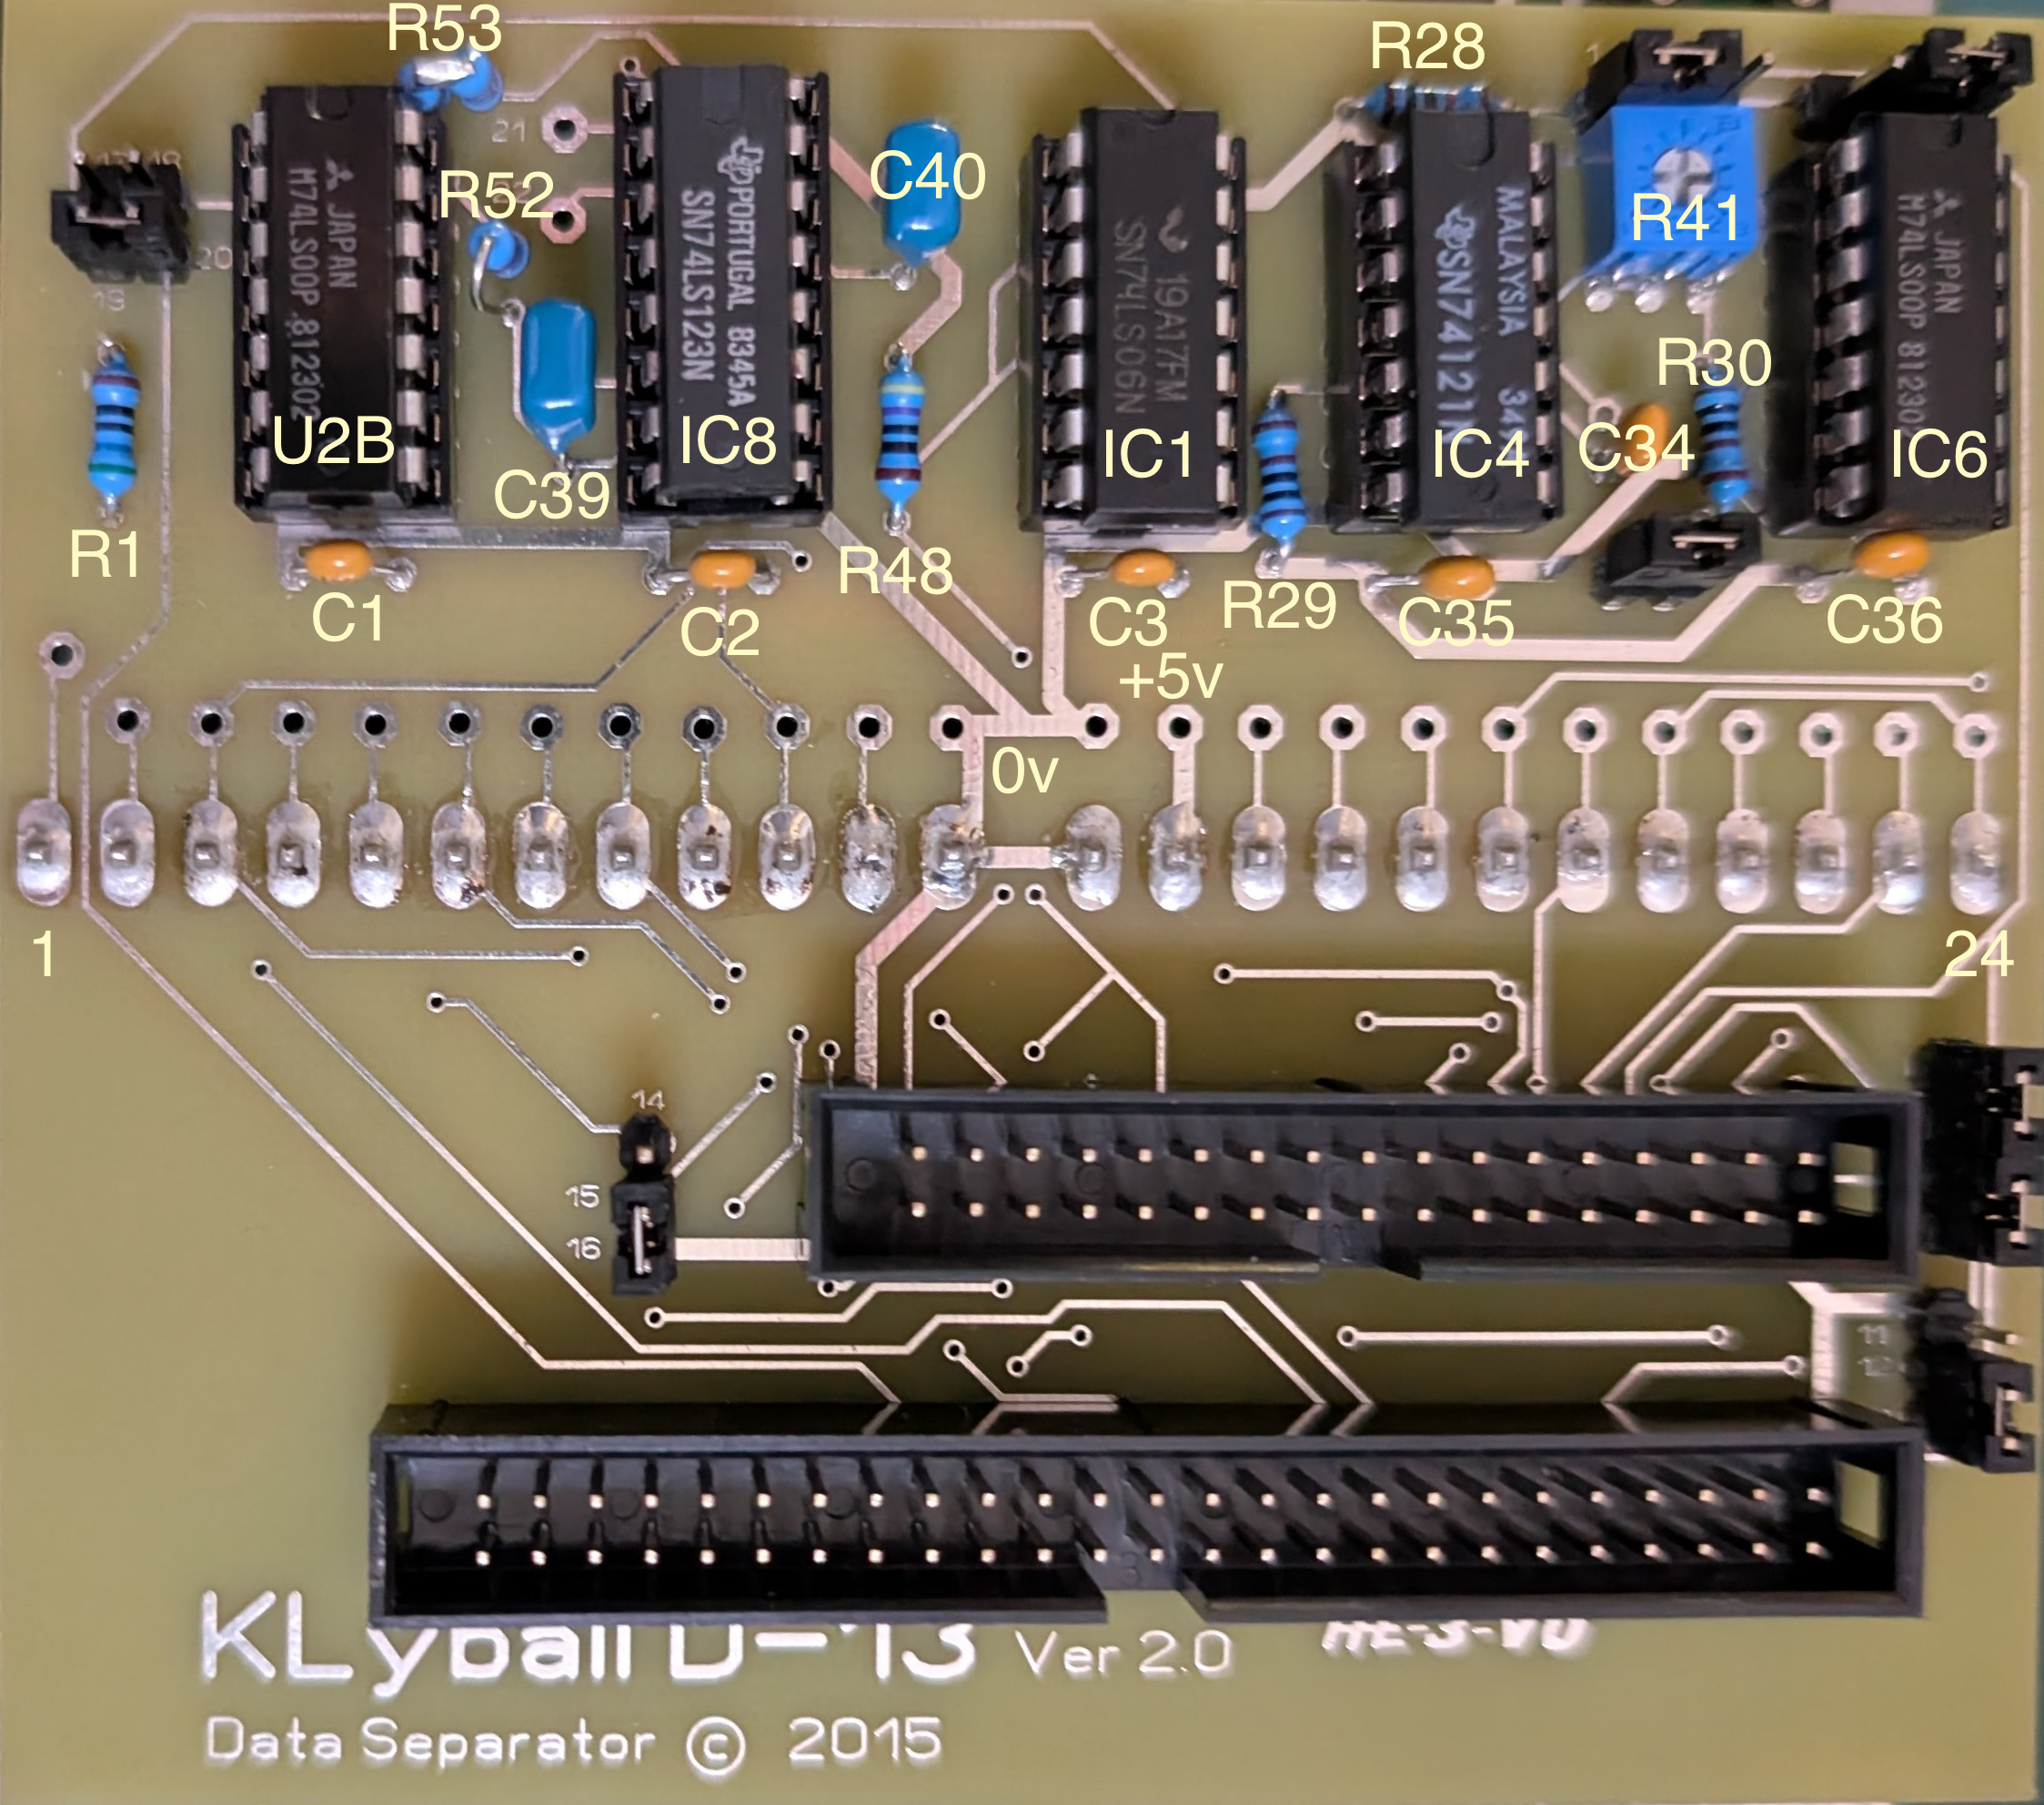
\includegraphics[width=3.5in]{images/D13Layout.jpg}
\caption{Component layout details.}
\label{fig:layout}
\end{center}
\end{figure}

\section{Power Connection}

Ensure that there is +5 supplied to pin 14 of the connector on the 610 expansion board. This may require a small jumper be added from +5V to this pin. See \textbf{Fig. \ref{fig:powerjumper}} for details.

\begin{figure}[htbp]
\begin{center}
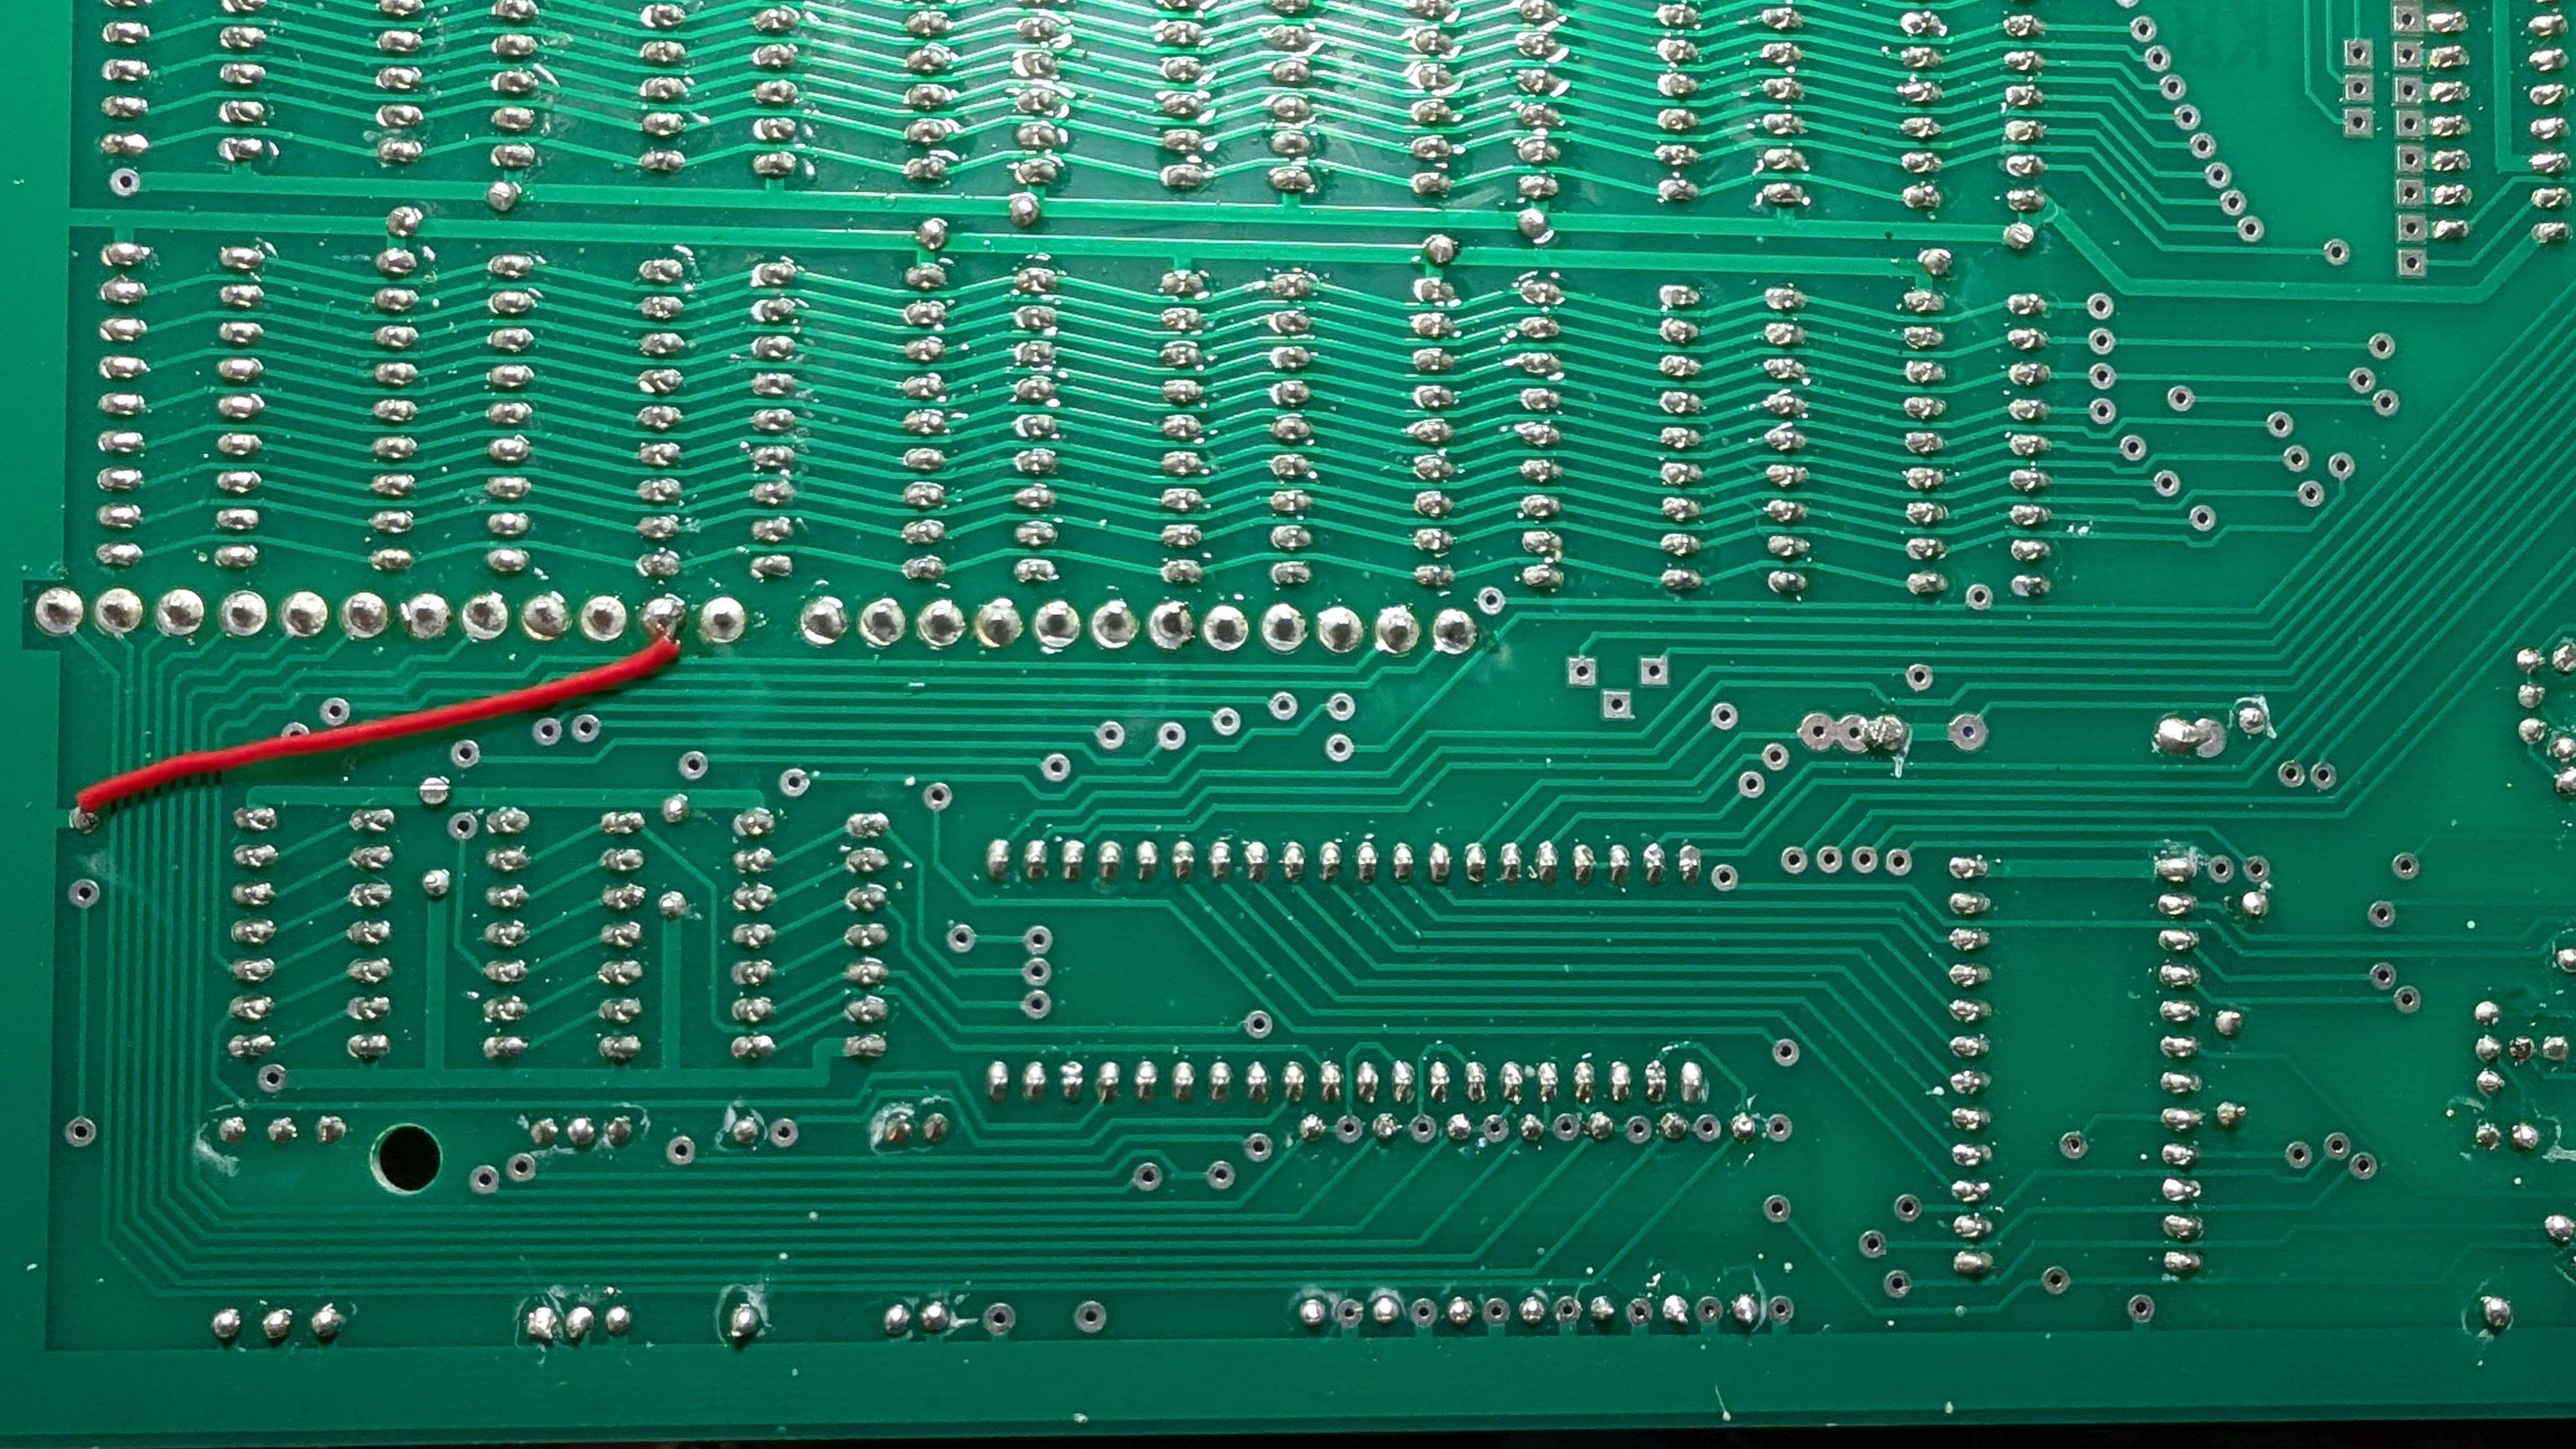
\includegraphics[width=3.5in]{images/PowerJumper}
\caption{Adding a power connection.}
\label{fig:powerjumper}
\end{center}
\end{figure}

